\section{Durchführung und Auswertung}

\subsection{LABVIEW-Messprogramm}

Wir haben zur Messung das bereits vorhandene Messprogramm verwendet. Allerdings zeigte sich im Laufe der Messungen, dass die Qualität gesteigert werden kann, wenn zwischen den einzelnen Messungen die Hochspannung auf $0V$ heruntergefahren wird. Durch das Methan können dann verbleibende Ionen anscheinend besser herausgespült werden. Daher haben wir das Programm um diese "`Reinigungsphase"' erweitert.

\subsection{Einstellen der Messelektronik}
Nachdem wir eine \atom{238}{}{U}-Probe einsetzten, machten wir uns mit der Messelektronik vertraut, indem wir das Signal am Oszilloskop betrachten.
\begin{itemize}
 \item Nach dem Vorverstärker sehen wir ein hochfrequentes Signal mit aufmodulierten Pulsen
 \item Nach dem Hauptverstärker sehen wir Peaks, deren Amplitude wir einstellen können indem wir den Verstärkungsfaktor verändern. Wir wählen eine 50-fache Verstärkung und eine Shaping-Zeit von $6\mu s$ und erhalten Peaks mit einer Amplitude $U = -8V$ und einer Abklingzeit von $t = 16\mu s$.
 \item Am SCA (Single Channel Analyzer) haben wir die untere Diskriminatorschwelle auf $0.3$ eingestellt. Sie dient dazu, das Rauschen vom eigentlichen Signal zu trennen, so dass nur wirkliche Zerfälle gezählt werden. 
\end{itemize}

\subsection{Zählrohrcharakteristik}

Wir haben damit begonnen, die Zählrohrcharakteristik aufzunehmen. Dazu haben wir eine \atom{238}{}{U} Probe verwendet, die eine gute Zählrate zeigt.

\begin{figure}[H]
 \centering 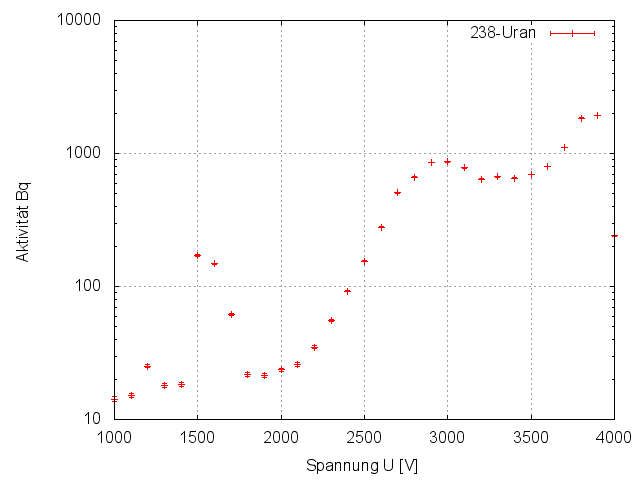
\includegraphics[width=0.9\linewidth]{Messwerte/plots/U238.png}
 \caption{Zählrohrcharakteristik, gemessen mit \atom{238}{}{U}}
\end{figure}
Als Parameter haben wir dabei gesetzt: $U = 1kV \cdots 4kV$, $\Delta U = 100 V$, $t = 50s$ sowie $t_{Pause} = 10s$. Die Fehler in diesem und allen weiteren Plots haben wir berechnet über $ S_n = \frac{\partial n}{\partial N} \cdot S_N = \frac{1}{t} \cdot \sqrt{N} = \sqrt{\frac{n}{t}}$.

Der Graph zeigt den erwarteten Verlauf, abgesehen von einigen Ausreisern am Anfang des $\alpha$-Plateaus. \atom{238}{}{U} zerfällt durch $\alpha$-Zerfall in \atom{234}{}{Th} (Thorium). Dieses zerfällt mit einer Halbwertszeit $T_{1/2} = 24.10d$ durch einen $\beta^-$-Zerfall in \atom{234}{}{Pa} (Proactinium), welches ebenfalls durch $\beta^-$-Zerfall in \atom{234}{}{U} zerfällt. Deshalb sehen wir in der Zählrohrcharakteristik sowohl ein Plateaubereich, in dem haupsächlich $\alpha$-Strahlung detektiert wird bei ca. $U = 1100V$ bis $U = 2100V$ als auch einen Plateaubereich in dem $\alpha$- und $\beta$-Strahlung detektiert werden zwischen $3000V$ und $3700V$.

Auf das Abziehen des Untergrundes haben wir verzichtet, einerseits da der Untergrund eine Aktivität von ca. $0.001Bq$ bis maximal $1.0Bq$ zeigte, also deutlich weniger als die eigentliche Intensität. Andererseits sind die Ergebnisse der Untergrundmessung eh fraglich, wie später erleutert wird.

\subsection{Bestimmung der Halbwertszeit von \atom{147}{}{Sm} ($\alpha$-Zerfall)}

Wir haben für den im voherigen Versuchsabschnitt ermittelten $\alpha$-Plateaubereich eine grobe Messung mit einer \atom{147}{}{Sm}-Probe vorgenommen. Die Parameter dafür waren: $U= 1000V \cdots 3300V$, in $\Delta U = 100 V$ Schritten mit $t=200s$ und $t_{Pause} = 10s$.

\begin{figure}[H]
 \centering 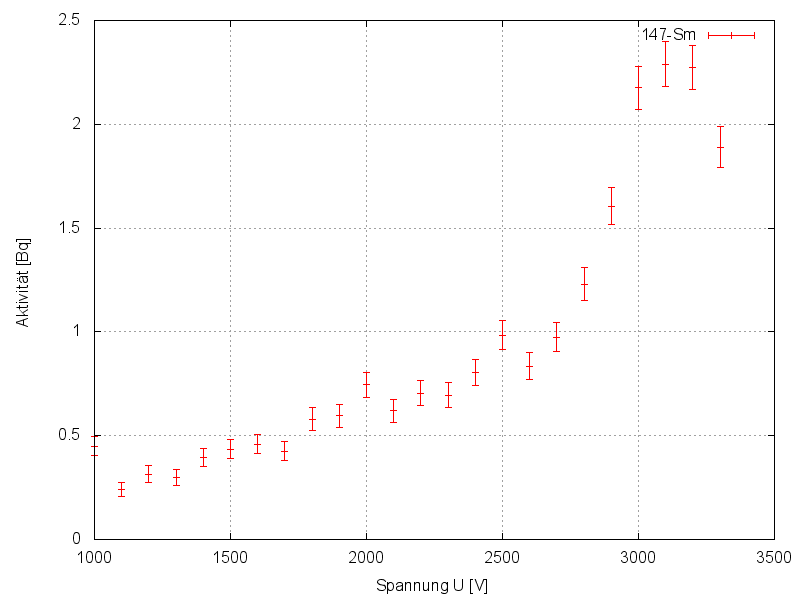
\includegraphics[width=0.9\linewidth]{Messwerte/plots/Sm147_plateau.png}
 \caption{Plateaubereich, gemessen mit \atom{147}{}{Sm}}
\end{figure}

Die Mitte des Plateaus liegt also bei etwa $U_{\alpha} = 2000\ V$. Bei dieser Spannung betrug die Zählrate $n = 0.745\ Bq$, die durchschnittliche Zählrate auf dem Plateau lag aber eher bei $\overline{n} = 0.6\ Bq$, so dass wir zur Abschätzung der benötigten Messzeit diesen Wert verwendet haben. Über die Gleichung \ref{zeitfuerkleinenfehler} ermitteln wir, dass unsere Messung mindestens $t_{0.02} = 4168\ s$ dauern sollte. Wir führen daher eine Messung mit $t = 4200\ s$ und $ U = 2000\ V$ durch. Dabei erhalten wir eine Zählrate von $n = 0.39\ Bq$. Diese Zählrate ist wesentlich niedriger als der von uns erwartete Wert und kann auch nur sehr schwer durch statistische Schwankungen begründet werden. Auch zwei kürzere ($t = 60s$) Kontrollmessungen ergeben wieder deutlich höhere Zählraten ($n_1 = 0.650\ Bq$ und $n_2 = 0.633\ Bq$). Als Hauptfehlerquellen stuffen wir die Gaszufuhr und die Hochspannung ein. Bei genauerem Betrachten der Gasableitung ist uns dann aufgefallen, dass sich im Schlauch das Gas in Form von Blasen fortbewegt. Also haben wir den Schlauch entfernt und festgestellt, dass er mit Öl (und \atom{40}{}{K}-Krümmeln) gefüllt war, welches vermutlich aus dem Bläschenzähler stammt, durch zu hohe Gaszufuhr mitgerissen wurde und sich im Schlauch wieder ablagerte. Nach Reinigung des Schlauches war der Abfluss des Gases nun wieder deutlich konstanter. Wir führten also erneut eine Messung mit $t=4200s$ durch und erhielten diesmal eine realistischere Zählrate von $n = (0,611 \pm 0.012) Bq$ (also $N = 2565$). Für die Untergrundkorrektur haben wir den Messwert bei $U = 1950V$ verwendet, die Zählrate betrug dort $n_{Untergrund} = 0.004 Bq$.

Für die Berechnung der Halbwertszeit $t_{1/2}$ haben wir weiterhin den Innendurchmesser der Aluschale gemessen und $d = (29.125 \pm 0.125) mm$ erhalten. Die Oberfläche der Probe beträgt somit $F = \frac{\pi}{4} d^2 = (666.2 \pm 5.7) mm^2$.

Die Halbwertszeit können wir nun berechnen:

\begin{align}
 T_{1/2} \left( \atom{147}{}{Sm} \right) &= \frac{\ln 2 \cdot R_{Sm_2O_3} \cdot \rho_{Sm_2O_3} \cdot N_A \cdot h_{rel} \cdot F}{2 \cdot n \cdot m_{rel,Sm_2O_3}} \\
 & = 3.62\cdot 10^{17} \cdot \frac{6.66cm^2}{0.611 Bq - 0.004 Bq} \\
 & = (1.260 \pm 0.026) \cdot 10^11 a
\end{align}

Die Literaturangabe für die Halbwertszeit beträgt $T_{1/2 - lit} \left( \atom{147}{}{Sm} \right) = 1.06 \cdot 10^11 a$. Unser Ergebnis liegt also innerhalb von 8 Standardabweichungen über dem erwarteten. Dies deutet auf systematische Fehler hin, die wir eher nicht bei der Messung des Durchmessers vermuten. Die Ursache der Abweichung muss also in der Zählrate liegen, diese war anscheinend zu gering. Mögliche Ursachen hierfür sind eine zu hoch eingestellte Diskriminatorschwelle, ein zu starker Gasfluss, eine zu niedrige Spannung sowie bauartbedingte Einflüße, wie zB ein zu großer Abstand zwischen Probe und Draht. Letzteres war durch uns nicht beeinflussbar. Die gewählte Diskriminatorschwelle sowie der Gasfluss erschienen uns allerdings nötig, da die Zählrate wie bereits erwähnt oft in unrealistische Bereiche ging und ein Senken der Schwelle bzw eine Verringerung des Gasflusses diese Störeffekte nur noch weiter verstärkt hätte.  

\subsection{Halbwertszeit von \atom{40}{}{K} ($\beta$-Zerfall) - Teil 1}

Für die Messung der Halbwertszeit von \atom{40}{}{K} haben wir das $\beta$-Plateau im Bereich von $U = 2900\ V \cdots\ 4000\ V$ in $\Delta U = 100 V$-Schritten je $t=100s$ lang vermessen. Dazu verwendeten wir $m=1.2158g$ Kalium.

\begin{figure}[H]
 \centering 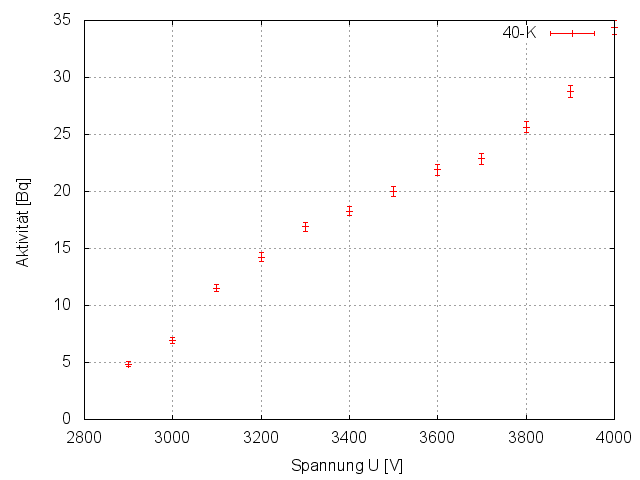
\includegraphics[width = 0.99\linewidth]{Messwerte/plots/K40_plateau.png}
 \caption{\atom{40}{}{K}-Plateau}
 \label{k40plateau}
\end{figure}

Die Mitte des Plateaus liegt also wie in Abb \ref{k40plateau} sichtbar bei etwa $U = 3600V$, wobei die Zählrate dort etwa $n = 22 Bq$ beträgt. Daraus ergibt sich eine minimale Messdauer von $t_{0.02} = 113.6 s$. Wir haben also die bereits für die Plateaumessung verwendete Probe mit $m = 1.2158g$ nochmals für $t = 120s$ vermessen. Dabei erhielten wir in zwei Messungen Zählraten von $n_1 = 9620.017 Bq$ bzw. $n_2 = 31 202.083 Bq$. Diese unrealistischen Werte könnten z.B. durch Übergang in den Gasentladungsmodus, Verbleiben von Ionen im Zählrohr, eine zu niedrig eingestellte Diskriminatorschwelle oder Defekte der Messelektronik/Software entstehen. Bei einer dritten Messung, nach einem Reset der Spannung, gelang uns wieder eine vernünftige Messung mit einer Zählrate $n = 5.708 Bq$. Da diese jedoch der Plateaumessung deutlich widersprach, haben wir diese ebenfalls wiederholt. Dabei haben wir wieder $U = 2900V \cdots 4000V$ in $\Delta U = 100 V$-Schritten je $t=100s$ als Parameter verwendet. 
Für die minimale Messdauer erhalten wir nun $t_{0.02} = 452.08 s$.

\begin{figure}[H]
 \centering 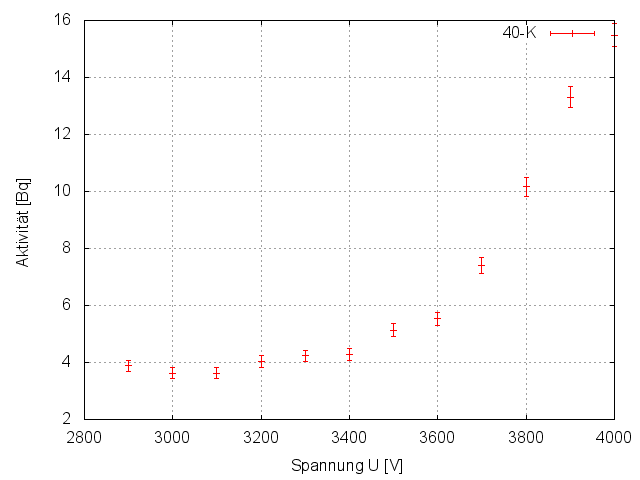
\includegraphics[width = 0.99\linewidth]{Messwerte/plots/K40_plateau2.png}
 \caption{\atom{40}{}{K}-Plateau}
\end{figure}

\subsection{Untergrundmessung}
Über das Wochenende haben wir eine ausführliche Untergrundmessung vorgenommen. Dazu haben wir das angepasste Messprogramm verwendet, und Messungen von $U = 0V \cdots 4000V$ mit $\Delta U = 50V$. Die Dauer der Einzelmessungen stellten wir auf $t=3000s$ mit einer Pause von $t_{Pause} = 60 s$ sowie einer gleichlangen Zeit für das Einstellen der Spannung.

\begin{figure}[H]
 \centering 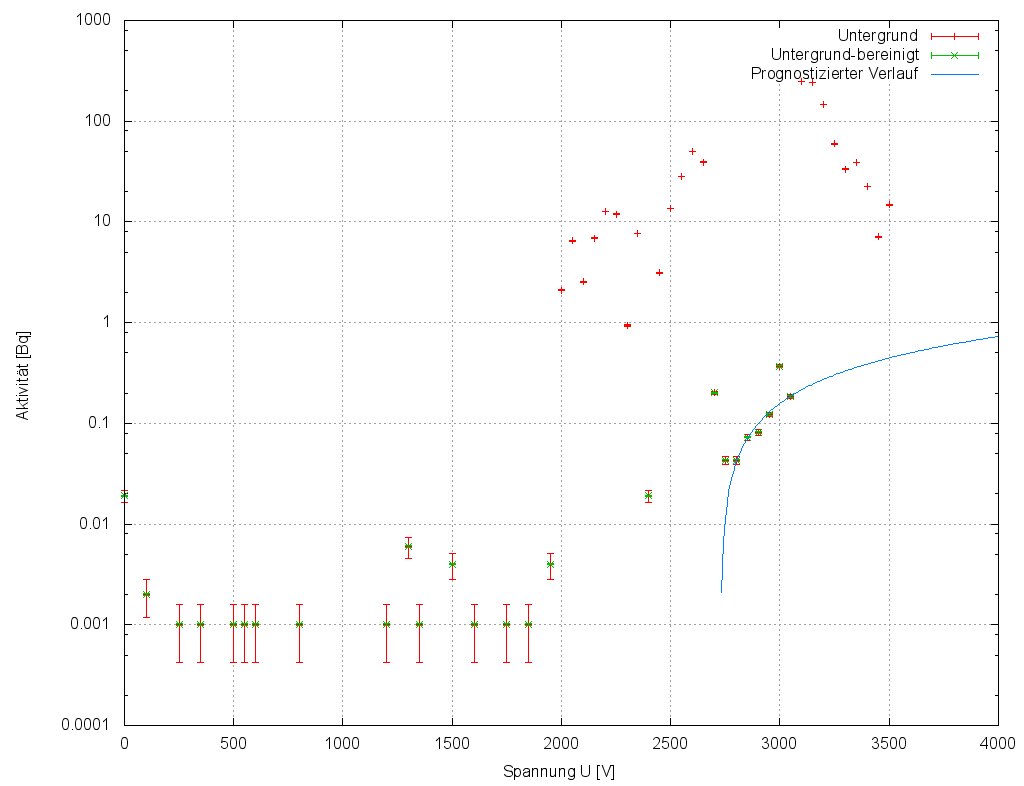
\includegraphics[width = 0.99\linewidth]{Messwerte/plots/untergrund_we_bereinigt.png}
 \caption{Untergrundmessung}
\end{figure}


Am Montag mussten wir leider gleich mehrere Probleme feststellen. Erstens hatten wir uns verrechnet, die Messung wäre erst am Montag abend fertig gewesen. Zweitens war die Gaszufuhr versiegt, es waren trotz geöffnetem Hahn keine Blasen mehr zu sehen im Durchflusszähler und drittens waren die Zählraten häufig und ab ca 3400V dann konsequent zu hoch. Wir haben daher beschlossen, Zählraten mit $ n > 0.5 Bq$ zu verwerfen. Diese Grenze haben wir einerseits aus dem Vergleich mit den Messungen mit Präparat und andererseits aus den durchschnittlichen Untergrundmesswerten ermittelt.


\subsection{Halbwertszeit von \atom{40}{}{K} ($\beta$-Zerfall) - Teil 2}

Am Freitag hatten wir bereits die minimale Messdauer auf $t_{0.02} = 452.08 s$ bestimmt. Für die Untersuchung der \atom{40}{}{K}-Aktivität in Abhängigkeit von der Masse verwendeten wir also eine Messdauer von $t = 460s$ bei der Plateauspannung $U = 3600V$.
Nachdem die erste Messung erfolgreich war, bekammen wir bei weiteren nurnoch wesentlich zu hohe Zählraten. Daher haben wir die Diskriminatorschwelle am SCA von 0.3 auf 0.5 erhöht. Diese Veränderung reduziert natürlich die Vergleichbarkeit der Messergebnisse und erfordert eine erneute Messung des Untergrundes. Nach einigen erfolgreichen Messungen begannen die Probleme erneut,
diesmal stellte sich die Zählrate auf einen Wert um $n = 60 Bq$ ein. Wir versuchten dieses Phänomen durch weitere Messungen zu untersuchen.
Eine zu niedrige Diskriminatorschwelle können wir relativ sicher als Fehlerquelle ausschliessen, da die Zählraten kontinuirlich stiegen, selbst nachdem wir die Probe für eine Untergrundmessung entfernt haben. Als Ursachen kommen eher die üblichen Verdächtigen wie Verbleibende Ionen, Gasentladung sowie Defekte bei der Mess- und Steuerelektronik in Frage.
Ein Zusammenhang der Zählrate mit der Netzfrequenz von $f = 50Hz$ erscheint auch möglich. Insbesondere da die Kühlmaschiene des benachbarten Versuches nach einer Leckage von Herr Stützler geöffnet wurde und ab diesem Moment ohne Abschirmung lief.
Für eine genauere Untersuchung sowie eine erneute Messung verblieb leider keine Zeit, so dass wir die Auswertung basierend auf den sechs Messpunkten vor Auftreten der Probleme durchgeführt haben.

\begin{figure}
 \centering 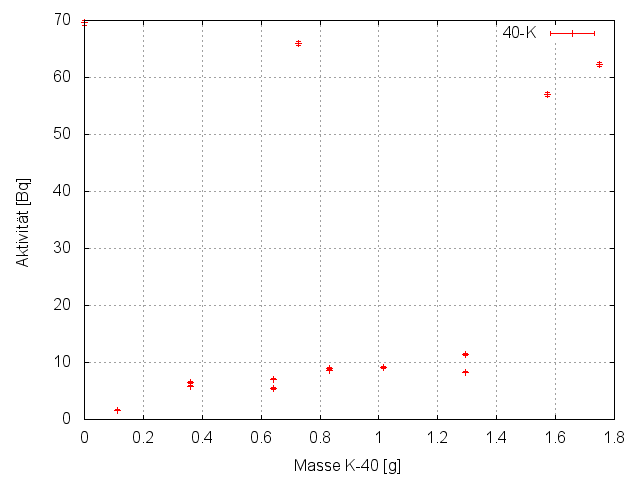
\includegraphics[width = 0.99\linewidth]{Messwerte/plots/K40_massenabh.png}
 \caption{Abhängigkeit der registrierten Aktivität von der Masse der Probe}
\end{figure}

\begin{figure}
 \centering 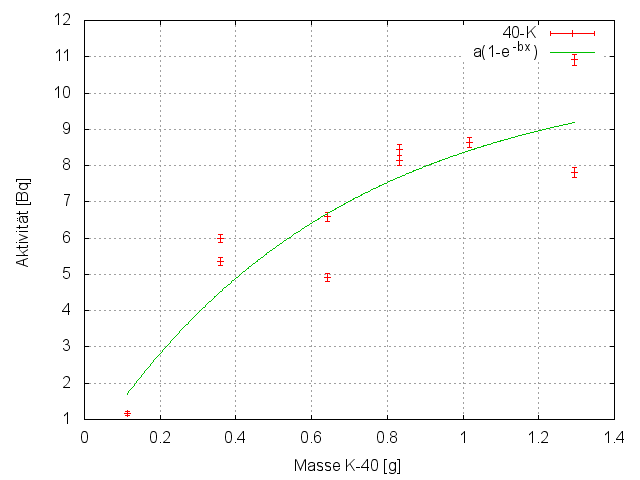
\includegraphics[width = 0.99\linewidth]{Messwerte/plots/K40_massenabh_bereinigt.png}
 \caption{Abhängigkeit der registrierten Aktivität von der Masse der Probe, unrealistische Messwerte wurden entfernt}
\end{figure}

Da uns die Untergrundmessung auf Grund der geschilderten Probleme misslang und die lange Untergrundmessung über das Wochenende den Bereich des $\beta$-Plateaus nicht abdeckt, haben wir eine Extrapolation vorgenommen. Die Daten der Untergrundmessung stützen diese allerdings nur sehr begrenzt ( $\chi^2 = 578.182$). Durch die Extrapolation erhalten wir eine Untergrundzählrate von $ n_{Untergrund} = 0.502 Bq$ für die Messungen bei $U = 3600V$.

Die massenabhängige Impulsrate ergibt sich aus
\begin{equation}
 n(m) = \frac{A_s \cdot F \cdot \rho}{\mu} \cdot \left( 1 - e^{-\frac{\mu \cdot m}{F \cdot \rho}} \right) = a \cdot \left( 1 - e^{-bm} \right)
\end{equation}
Da wir die Masse während der Messungen variert haben, können wir also diese Funktion an unsere bereinigten Messwerte fitten. Dabei erhalten wir die beiden Parameter
$$ a = (10.6341 \pm 2.138) Bq $$
$$ b = (1.54082 \pm  0.5996) $$

Die beiden Parameter sind antikorreliert mit $\rho_{ab} = -0.954$. Der hohe Wert für $\chi^2/DoF = 102.8$ zeigt uns, dass die Hauptfehlerursache nicht in der statistischen Verteilung der Zerfälle liegt, sondern durch sonstige experimentelle Einflüße ausgelöst wird. Die Ermittlung der Fehlerbalken im Diagramm aus der Zählrate unterschätzt also den wahren Fehler. 

Die Halbwertszeit können wir nun berechnen über
\begin{equation}
 T_{1/2}\left( \atom{40}{}{K} \right) = \frac{\ln 2}{1.13} \cdot \frac{f \cdot N_A \cdot h_{rel}}{2 \cdot a \cdot b \cdot m_{rel,KCl}}
\end{equation}
mit dem Fehler
\begin{equation}
 \left( \frac{S_{T_{1/2}}}{T_{1/2}} \right)^2 = \left( \frac{S_a}{a} \right)^2 + \left( \frac{S_b}{b} \right)^2 + 2 \cdot \rho_{ab} \cdot \frac{S_a}{a} \cdot \frac{S_b}{b}
\end{equation}

Somit erhalten wir $$T_{1/2} \left( \atom{40}{}{K} \right) = ( 0.730 \pm 0.151 ) \cdot 10^9 a$$

Der Literaturwert für die Halbwertszeit beträgt $T_{1/2} \left( \atom{40}{}{K} \right) = 1.277 \cdot 10^9 a$. Unser Ergebnis liegt also innerhalb von vier Standardabweichungen zum Literaturwert, scheint also einen leichten systematischen Fehler zu haben. Insbesondere sind die Zählraten geringfügig zu hoch, was entweder an einer zu niedrigen Diskriminatorschwelle oder an einer Unterschätzung des Untergrundes liegen kann. Beides erscheint durchaus wahrscheinlich, wir haben zwar die Schwelle nachjustiert, allerdings war sie möglicherweise immernoch nicht ausreichend hoch. Die Unterschätzung des Untergrundes ist sicher, da wir den Wert grob extrapoliert haben und uns dabei eher an der unteren Grenze orientiert haben. 